% Options for packages loaded elsewhere
\PassOptionsToPackage{unicode}{hyperref}
\PassOptionsToPackage{hyphens}{url}
\PassOptionsToPackage{dvipsnames,svgnames,x11names}{xcolor}
%
\documentclass[
  letterpaper,
  DIV=11,
  numbers=noendperiod]{scrartcl}

\usepackage{amsmath,amssymb}
\usepackage{lmodern}
\usepackage{iftex}
\ifPDFTeX
  \usepackage[T1]{fontenc}
  \usepackage[utf8]{inputenc}
  \usepackage{textcomp} % provide euro and other symbols
\else % if luatex or xetex
  \usepackage{unicode-math}
  \defaultfontfeatures{Scale=MatchLowercase}
  \defaultfontfeatures[\rmfamily]{Ligatures=TeX,Scale=1}
\fi
% Use upquote if available, for straight quotes in verbatim environments
\IfFileExists{upquote.sty}{\usepackage{upquote}}{}
\IfFileExists{microtype.sty}{% use microtype if available
  \usepackage[]{microtype}
  \UseMicrotypeSet[protrusion]{basicmath} % disable protrusion for tt fonts
}{}
\makeatletter
\@ifundefined{KOMAClassName}{% if non-KOMA class
  \IfFileExists{parskip.sty}{%
    \usepackage{parskip}
  }{% else
    \setlength{\parindent}{0pt}
    \setlength{\parskip}{6pt plus 2pt minus 1pt}}
}{% if KOMA class
  \KOMAoptions{parskip=half}}
\makeatother
\usepackage{xcolor}
\setlength{\emergencystretch}{3em} % prevent overfull lines
\setcounter{secnumdepth}{-\maxdimen} % remove section numbering
% Make \paragraph and \subparagraph free-standing
\ifx\paragraph\undefined\else
  \let\oldparagraph\paragraph
  \renewcommand{\paragraph}[1]{\oldparagraph{#1}\mbox{}}
\fi
\ifx\subparagraph\undefined\else
  \let\oldsubparagraph\subparagraph
  \renewcommand{\subparagraph}[1]{\oldsubparagraph{#1}\mbox{}}
\fi

\usepackage{color}
\usepackage{fancyvrb}
\newcommand{\VerbBar}{|}
\newcommand{\VERB}{\Verb[commandchars=\\\{\}]}
\DefineVerbatimEnvironment{Highlighting}{Verbatim}{commandchars=\\\{\}}
% Add ',fontsize=\small' for more characters per line
\usepackage{framed}
\definecolor{shadecolor}{RGB}{241,243,245}
\newenvironment{Shaded}{\begin{snugshade}}{\end{snugshade}}
\newcommand{\AlertTok}[1]{\textcolor[rgb]{0.68,0.00,0.00}{#1}}
\newcommand{\AnnotationTok}[1]{\textcolor[rgb]{0.37,0.37,0.37}{#1}}
\newcommand{\AttributeTok}[1]{\textcolor[rgb]{0.40,0.45,0.13}{#1}}
\newcommand{\BaseNTok}[1]{\textcolor[rgb]{0.68,0.00,0.00}{#1}}
\newcommand{\BuiltInTok}[1]{\textcolor[rgb]{0.00,0.23,0.31}{#1}}
\newcommand{\CharTok}[1]{\textcolor[rgb]{0.13,0.47,0.30}{#1}}
\newcommand{\CommentTok}[1]{\textcolor[rgb]{0.37,0.37,0.37}{#1}}
\newcommand{\CommentVarTok}[1]{\textcolor[rgb]{0.37,0.37,0.37}{\textit{#1}}}
\newcommand{\ConstantTok}[1]{\textcolor[rgb]{0.56,0.35,0.01}{#1}}
\newcommand{\ControlFlowTok}[1]{\textcolor[rgb]{0.00,0.23,0.31}{#1}}
\newcommand{\DataTypeTok}[1]{\textcolor[rgb]{0.68,0.00,0.00}{#1}}
\newcommand{\DecValTok}[1]{\textcolor[rgb]{0.68,0.00,0.00}{#1}}
\newcommand{\DocumentationTok}[1]{\textcolor[rgb]{0.37,0.37,0.37}{\textit{#1}}}
\newcommand{\ErrorTok}[1]{\textcolor[rgb]{0.68,0.00,0.00}{#1}}
\newcommand{\ExtensionTok}[1]{\textcolor[rgb]{0.00,0.23,0.31}{#1}}
\newcommand{\FloatTok}[1]{\textcolor[rgb]{0.68,0.00,0.00}{#1}}
\newcommand{\FunctionTok}[1]{\textcolor[rgb]{0.28,0.35,0.67}{#1}}
\newcommand{\ImportTok}[1]{\textcolor[rgb]{0.00,0.46,0.62}{#1}}
\newcommand{\InformationTok}[1]{\textcolor[rgb]{0.37,0.37,0.37}{#1}}
\newcommand{\KeywordTok}[1]{\textcolor[rgb]{0.00,0.23,0.31}{#1}}
\newcommand{\NormalTok}[1]{\textcolor[rgb]{0.00,0.23,0.31}{#1}}
\newcommand{\OperatorTok}[1]{\textcolor[rgb]{0.37,0.37,0.37}{#1}}
\newcommand{\OtherTok}[1]{\textcolor[rgb]{0.00,0.23,0.31}{#1}}
\newcommand{\PreprocessorTok}[1]{\textcolor[rgb]{0.68,0.00,0.00}{#1}}
\newcommand{\RegionMarkerTok}[1]{\textcolor[rgb]{0.00,0.23,0.31}{#1}}
\newcommand{\SpecialCharTok}[1]{\textcolor[rgb]{0.37,0.37,0.37}{#1}}
\newcommand{\SpecialStringTok}[1]{\textcolor[rgb]{0.13,0.47,0.30}{#1}}
\newcommand{\StringTok}[1]{\textcolor[rgb]{0.13,0.47,0.30}{#1}}
\newcommand{\VariableTok}[1]{\textcolor[rgb]{0.07,0.07,0.07}{#1}}
\newcommand{\VerbatimStringTok}[1]{\textcolor[rgb]{0.13,0.47,0.30}{#1}}
\newcommand{\WarningTok}[1]{\textcolor[rgb]{0.37,0.37,0.37}{\textit{#1}}}

\providecommand{\tightlist}{%
  \setlength{\itemsep}{0pt}\setlength{\parskip}{0pt}}\usepackage{longtable,booktabs,array}
\usepackage{calc} % for calculating minipage widths
% Correct order of tables after \paragraph or \subparagraph
\usepackage{etoolbox}
\makeatletter
\patchcmd\longtable{\par}{\if@noskipsec\mbox{}\fi\par}{}{}
\makeatother
% Allow footnotes in longtable head/foot
\IfFileExists{footnotehyper.sty}{\usepackage{footnotehyper}}{\usepackage{footnote}}
\makesavenoteenv{longtable}
\usepackage{graphicx}
\makeatletter
\def\maxwidth{\ifdim\Gin@nat@width>\linewidth\linewidth\else\Gin@nat@width\fi}
\def\maxheight{\ifdim\Gin@nat@height>\textheight\textheight\else\Gin@nat@height\fi}
\makeatother
% Scale images if necessary, so that they will not overflow the page
% margins by default, and it is still possible to overwrite the defaults
% using explicit options in \includegraphics[width, height, ...]{}
\setkeys{Gin}{width=\maxwidth,height=\maxheight,keepaspectratio}
% Set default figure placement to htbp
\makeatletter
\def\fps@figure{htbp}
\makeatother

\KOMAoption{captions}{tableheading}
\makeatletter
\makeatother
\makeatletter
\makeatother
\makeatletter
\@ifpackageloaded{caption}{}{\usepackage{caption}}
\AtBeginDocument{%
\ifdefined\contentsname
  \renewcommand*\contentsname{Table of contents}
\else
  \newcommand\contentsname{Table of contents}
\fi
\ifdefined\listfigurename
  \renewcommand*\listfigurename{List of Figures}
\else
  \newcommand\listfigurename{List of Figures}
\fi
\ifdefined\listtablename
  \renewcommand*\listtablename{List of Tables}
\else
  \newcommand\listtablename{List of Tables}
\fi
\ifdefined\figurename
  \renewcommand*\figurename{Figure}
\else
  \newcommand\figurename{Figure}
\fi
\ifdefined\tablename
  \renewcommand*\tablename{Table}
\else
  \newcommand\tablename{Table}
\fi
}
\@ifpackageloaded{float}{}{\usepackage{float}}
\floatstyle{ruled}
\@ifundefined{c@chapter}{\newfloat{codelisting}{h}{lop}}{\newfloat{codelisting}{h}{lop}[chapter]}
\floatname{codelisting}{Listing}
\newcommand*\listoflistings{\listof{codelisting}{List of Listings}}
\makeatother
\makeatletter
\@ifpackageloaded{caption}{}{\usepackage{caption}}
\@ifpackageloaded{subcaption}{}{\usepackage{subcaption}}
\makeatother
\makeatletter
\@ifpackageloaded{tcolorbox}{}{\usepackage[many]{tcolorbox}}
\makeatother
\makeatletter
\@ifundefined{shadecolor}{\definecolor{shadecolor}{rgb}{.97, .97, .97}}
\makeatother
\makeatletter
\makeatother
\ifLuaTeX
  \usepackage{selnolig}  % disable illegal ligatures
\fi
\IfFileExists{bookmark.sty}{\usepackage{bookmark}}{\usepackage{hyperref}}
\IfFileExists{xurl.sty}{\usepackage{xurl}}{} % add URL line breaks if available
\urlstyle{same} % disable monospaced font for URLs
\hypersetup{
  pdftitle={Parsons\_Paper\_Register \#7},
  pdfauthor={Anna Zhou \& Sarah Edelson},
  colorlinks=true,
  linkcolor={blue},
  filecolor={Maroon},
  citecolor={Blue},
  urlcolor={Blue},
  pdfcreator={LaTeX via pandoc}}

\title{Parsons\_Paper\_Register \#7}
\author{Anna Zhou \& Sarah Edelson}
\date{2023-02-13}

\begin{document}
\maketitle
\ifdefined\Shaded\renewenvironment{Shaded}{\begin{tcolorbox}[interior hidden, enhanced, frame hidden, breakable, boxrule=0pt, sharp corners, borderline west={3pt}{0pt}{shadecolor}]}{\end{tcolorbox}}\fi

\hypertarget{how-many-days-in-a-pay-period}{%
\subsection{How many days in a pay
period?}\label{how-many-days-in-a-pay-period}}

\begin{itemize}
\item
  The Parsons Paper Company register comprises monthly pay periods from
  January 1861-April 1869
\item
  Pay periods appear to be a month long with employees typically getting
  paid on the 1st of the next (?) month
\item
  Based off the spreadsheet from p.~253, most employees work between
  20-30 days each pay period, the average is around 27 so most employees
  work at least 6 days/week

  \begin{itemize}
  \item
    In Chapter IV of Green's book, she writes that male Holyoke paper
    makers worked 58-72 hours a week

    \begin{itemize}
    \tightlist
    \item
      11.25 hours five days a week + 8.75 hours on Saturday was typical
      for Holyoke textile mills
    \end{itemize}
  \item
    Women worked slightly shorter hours
  \end{itemize}
\item
  Pgs. 261-263 appear to comprise an entire pay period for the month of
  April in 1868 (most pay periods span \textasciitilde3 pages in the
  register)

  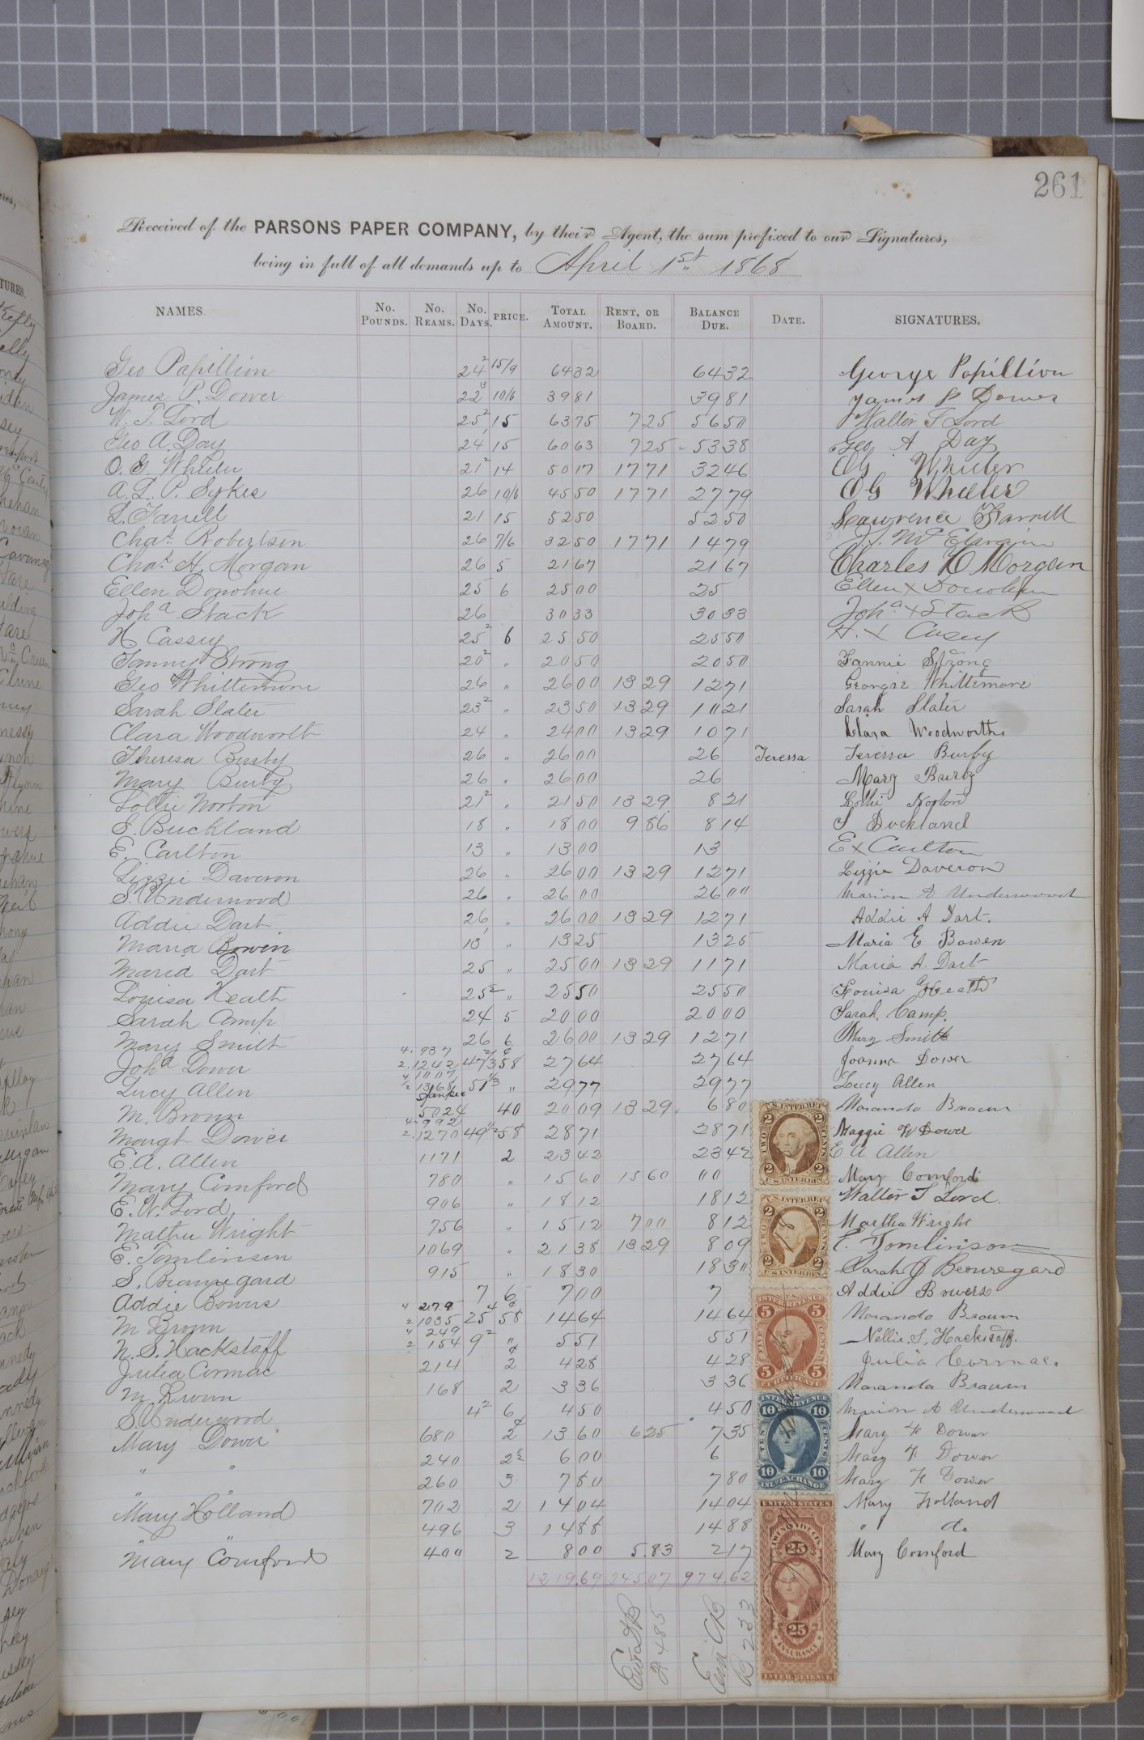
\includegraphics[width=2.29167in,height=\textheight]{images/Screenshot 2023-02-13 at 4.08.16 PM.png}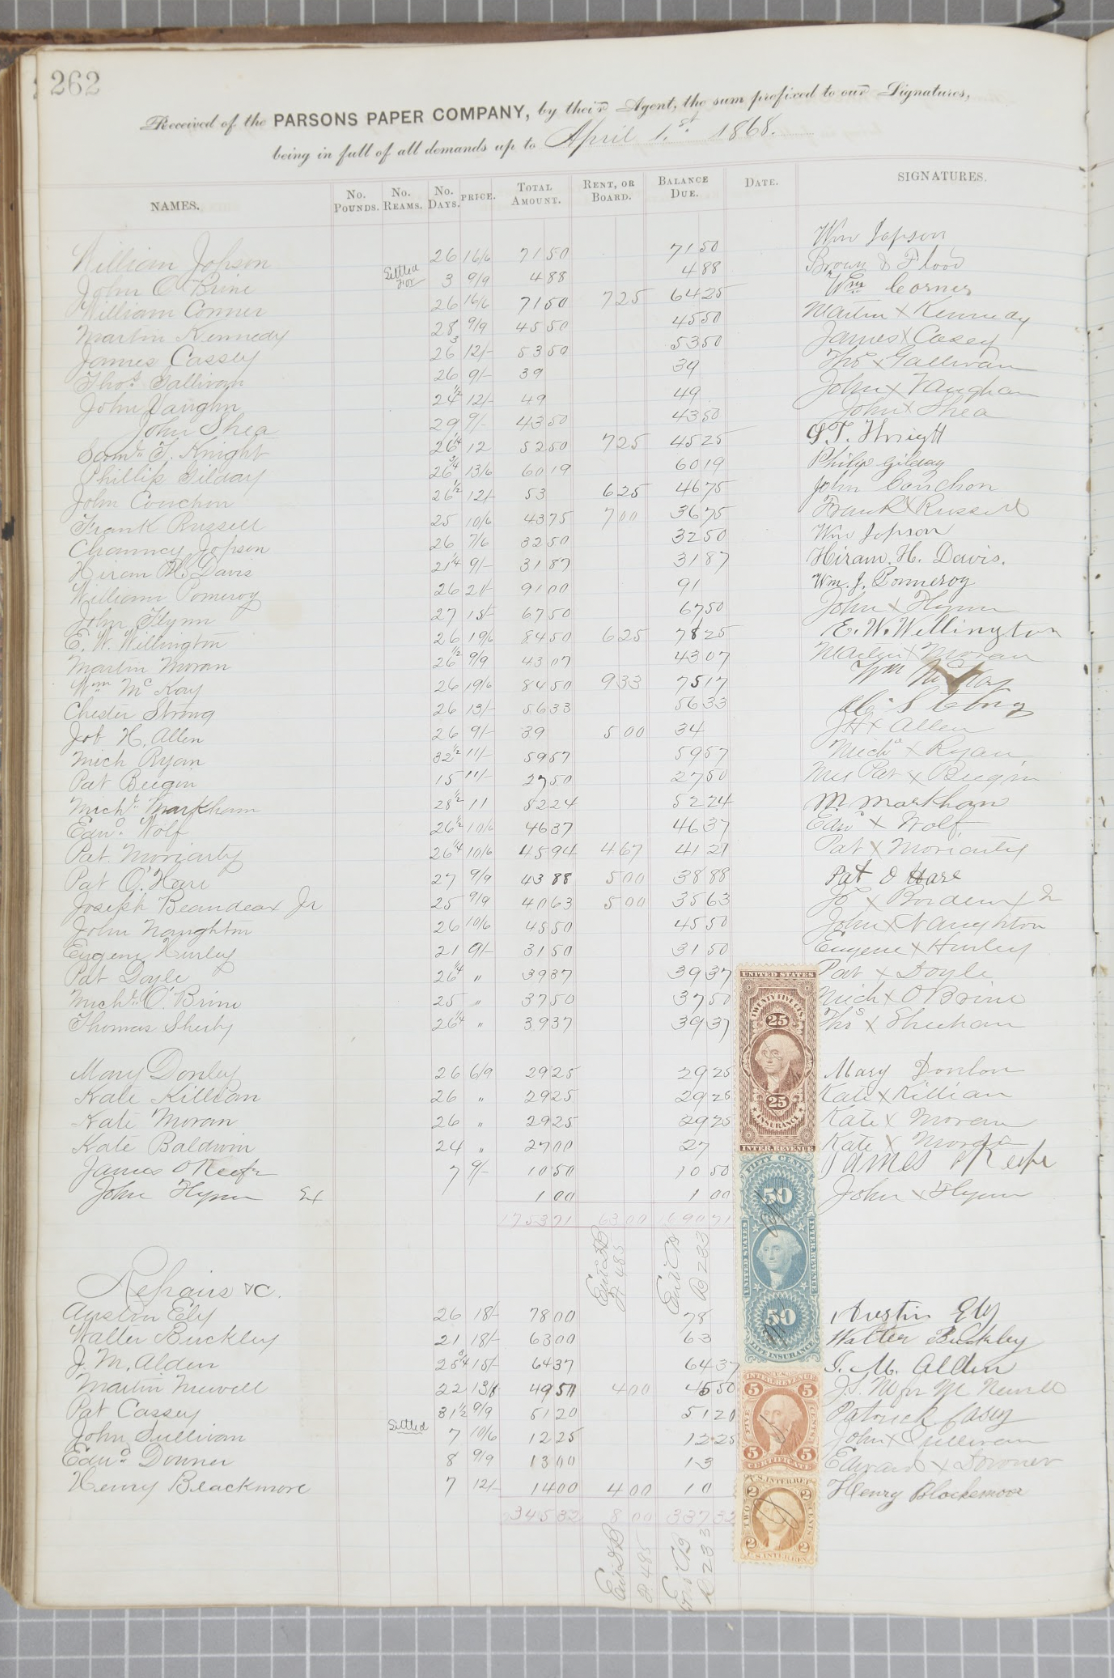
\includegraphics[width=2.29167in,height=\textheight]{images/Screenshot 2023-02-13 at 4.08.28 PM.png}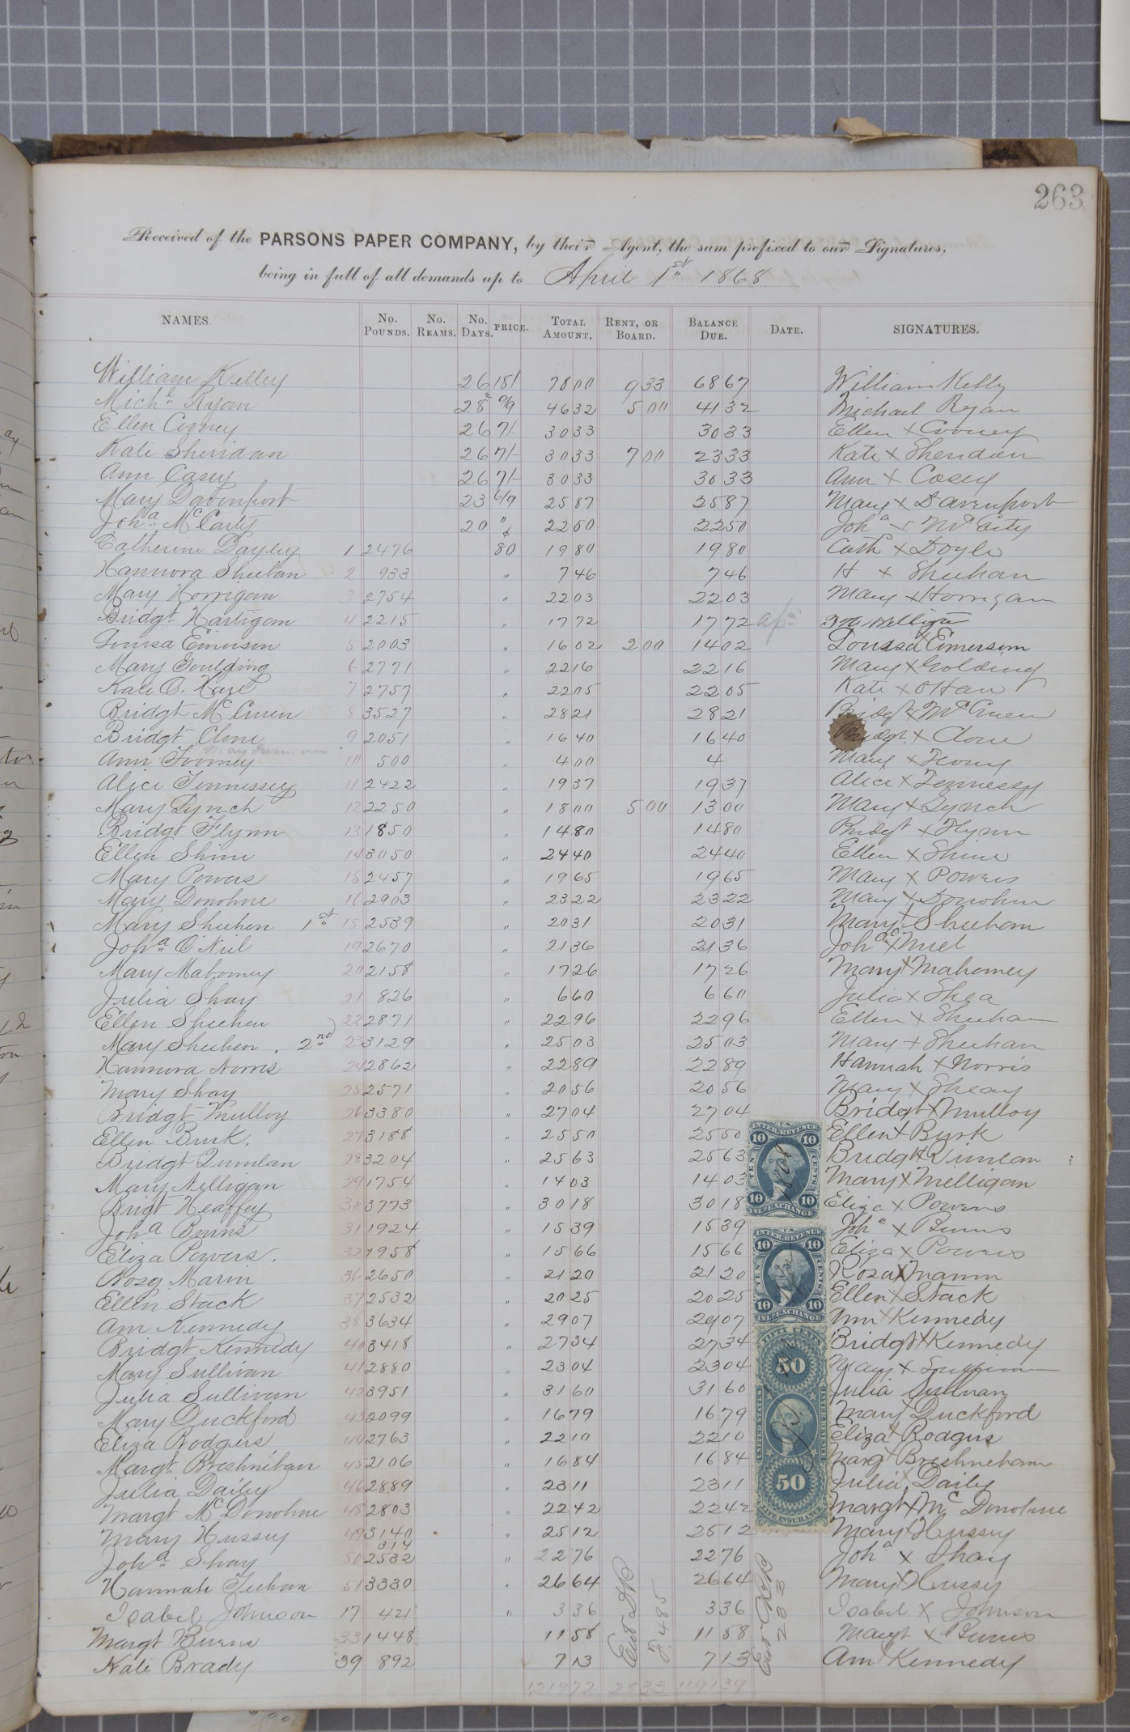
\includegraphics[width=2.29167in,height=\textheight]{images/Screenshot 2023-02-13 at 4.08.37 PM.png}
\item
  Pgs. 223-225 below and Pgs. 261-263 above are exactly one year apart
  in the register (April 1st 1867 + April 1st 1868)

  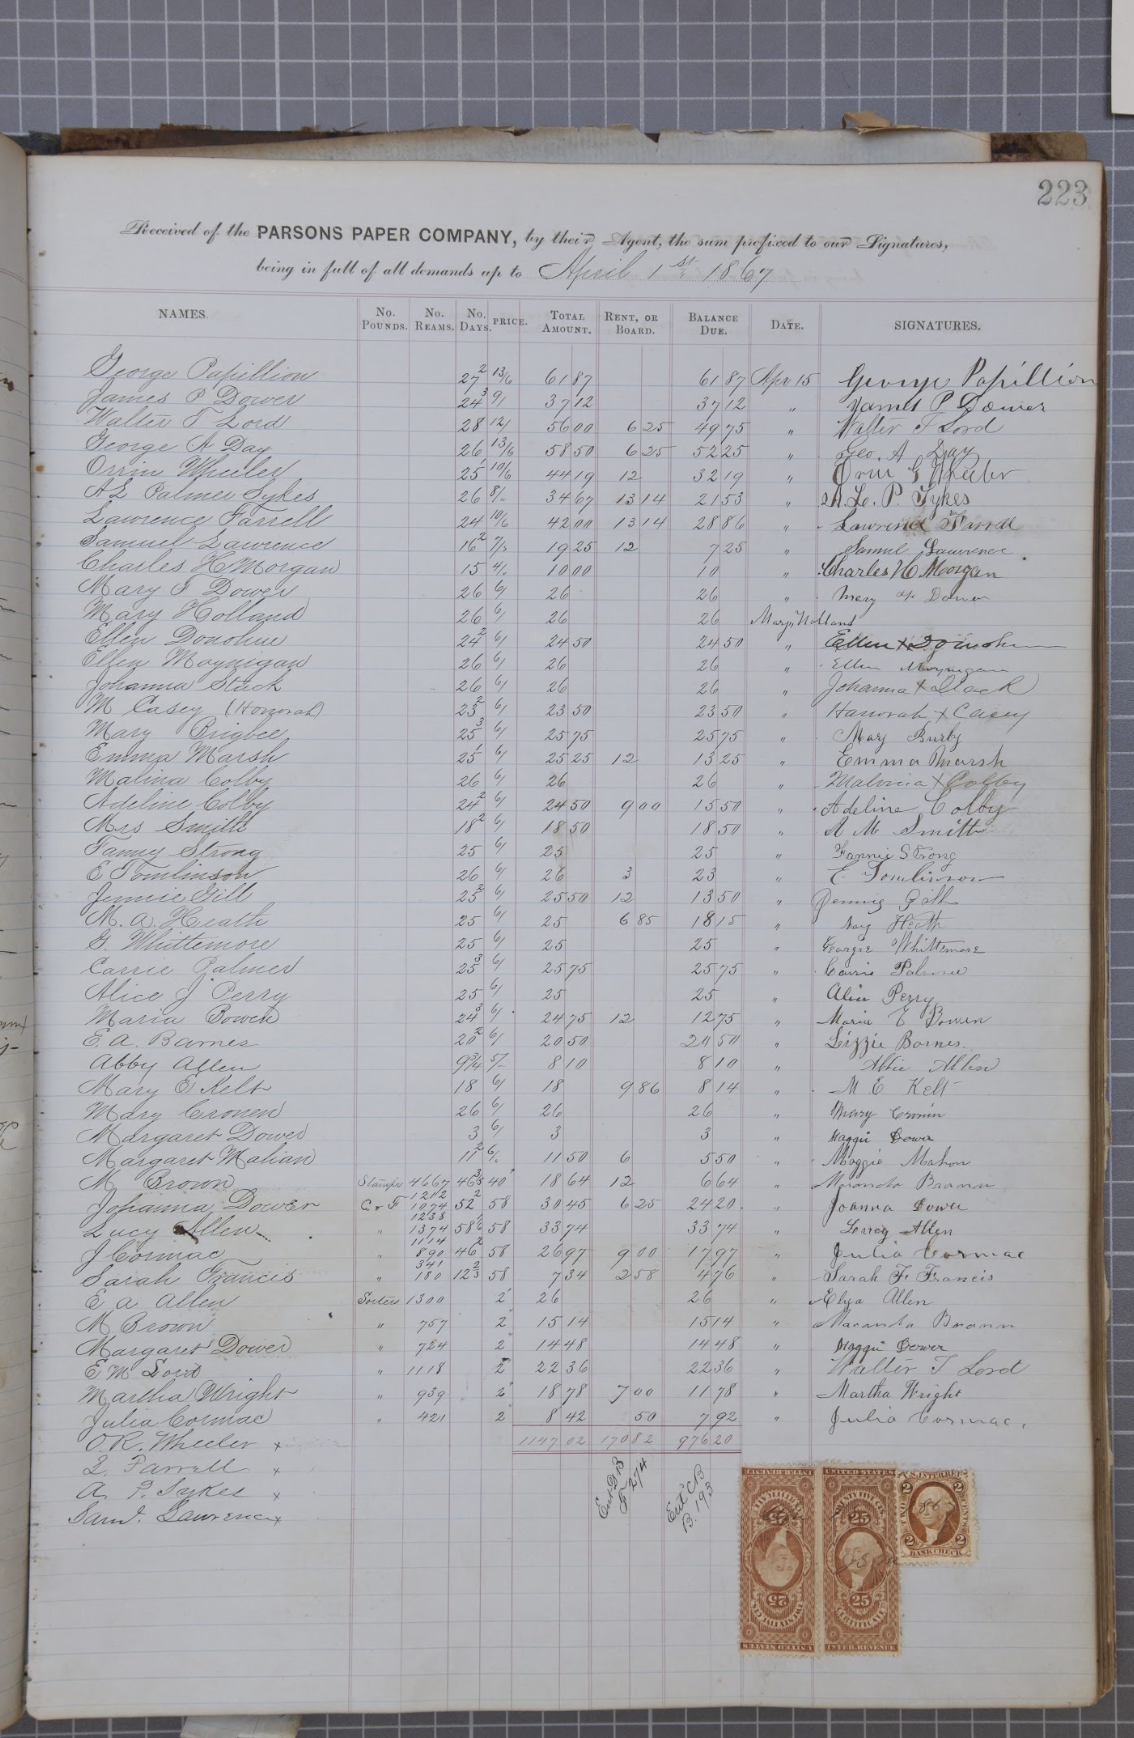
\includegraphics[width=2.29167in,height=\textheight]{images/Screenshot 2023-02-13 at 4.14.02 PM.png}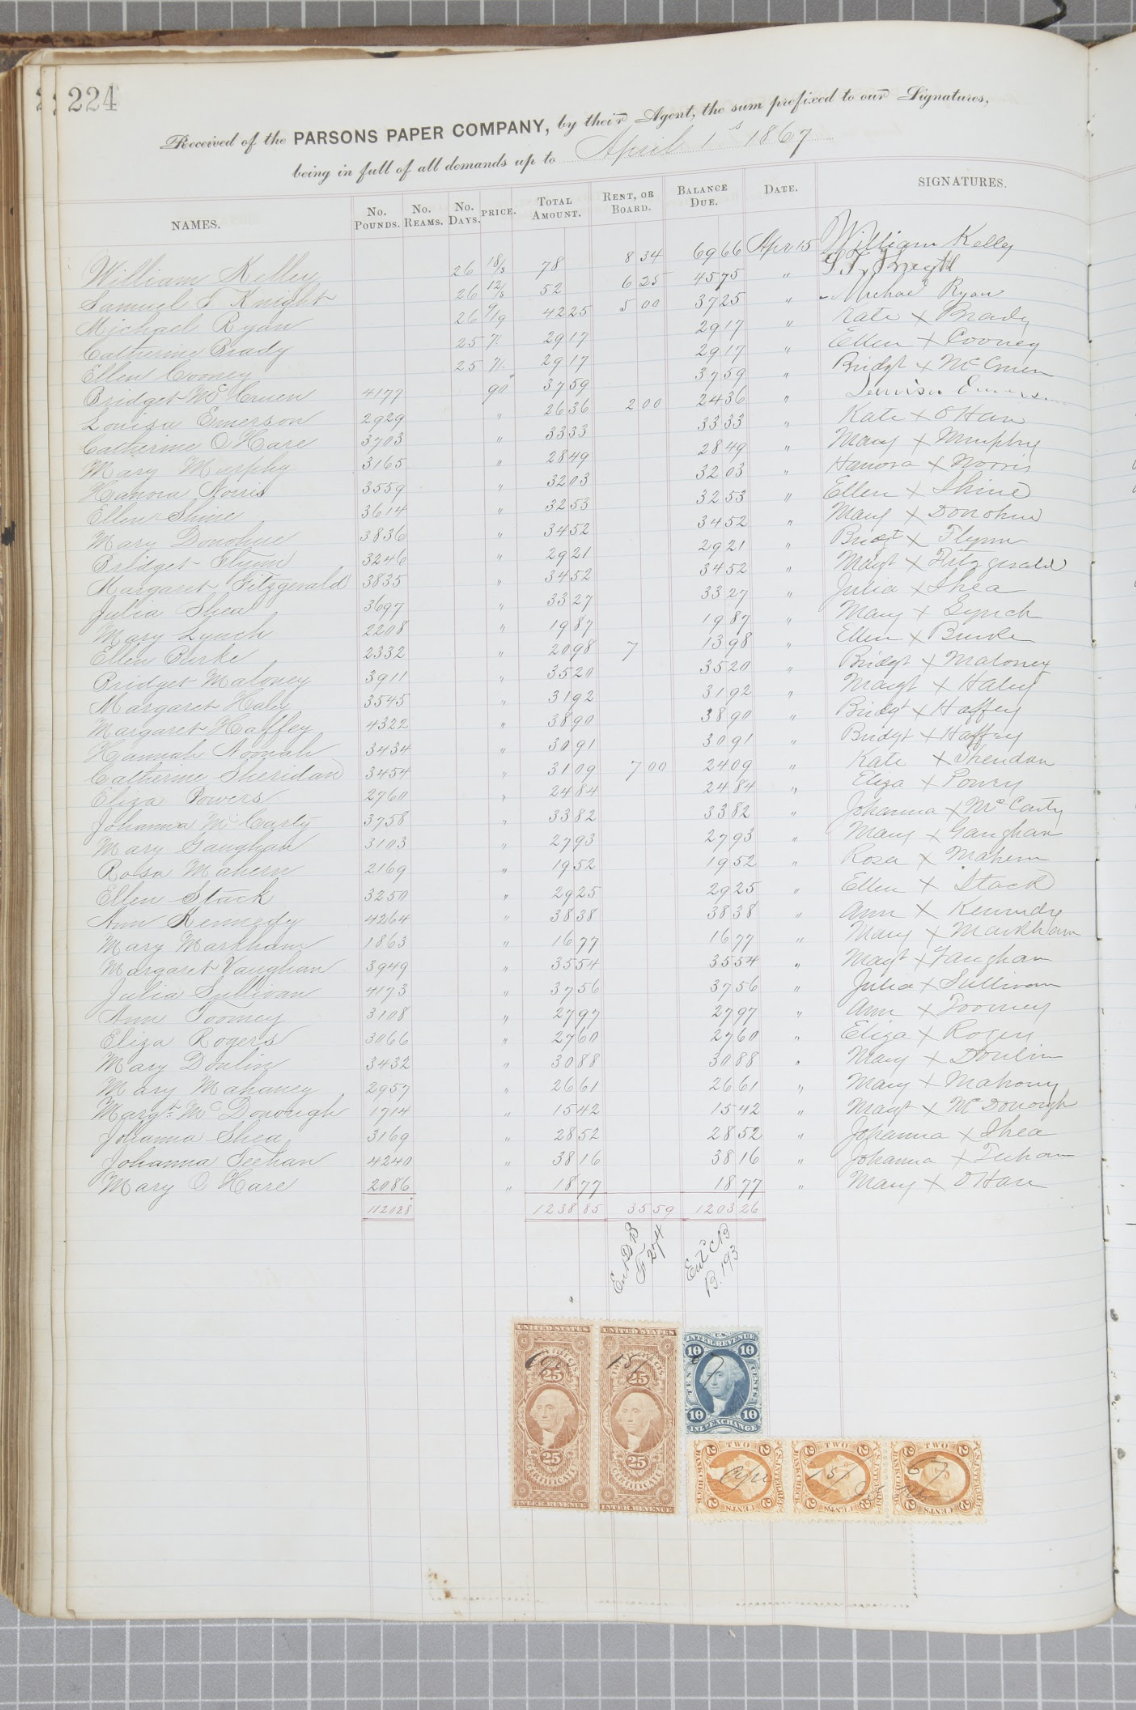
\includegraphics[width=2.29167in,height=\textheight]{images/Screenshot 2023-02-13 at 4.14.09 PM-01.png}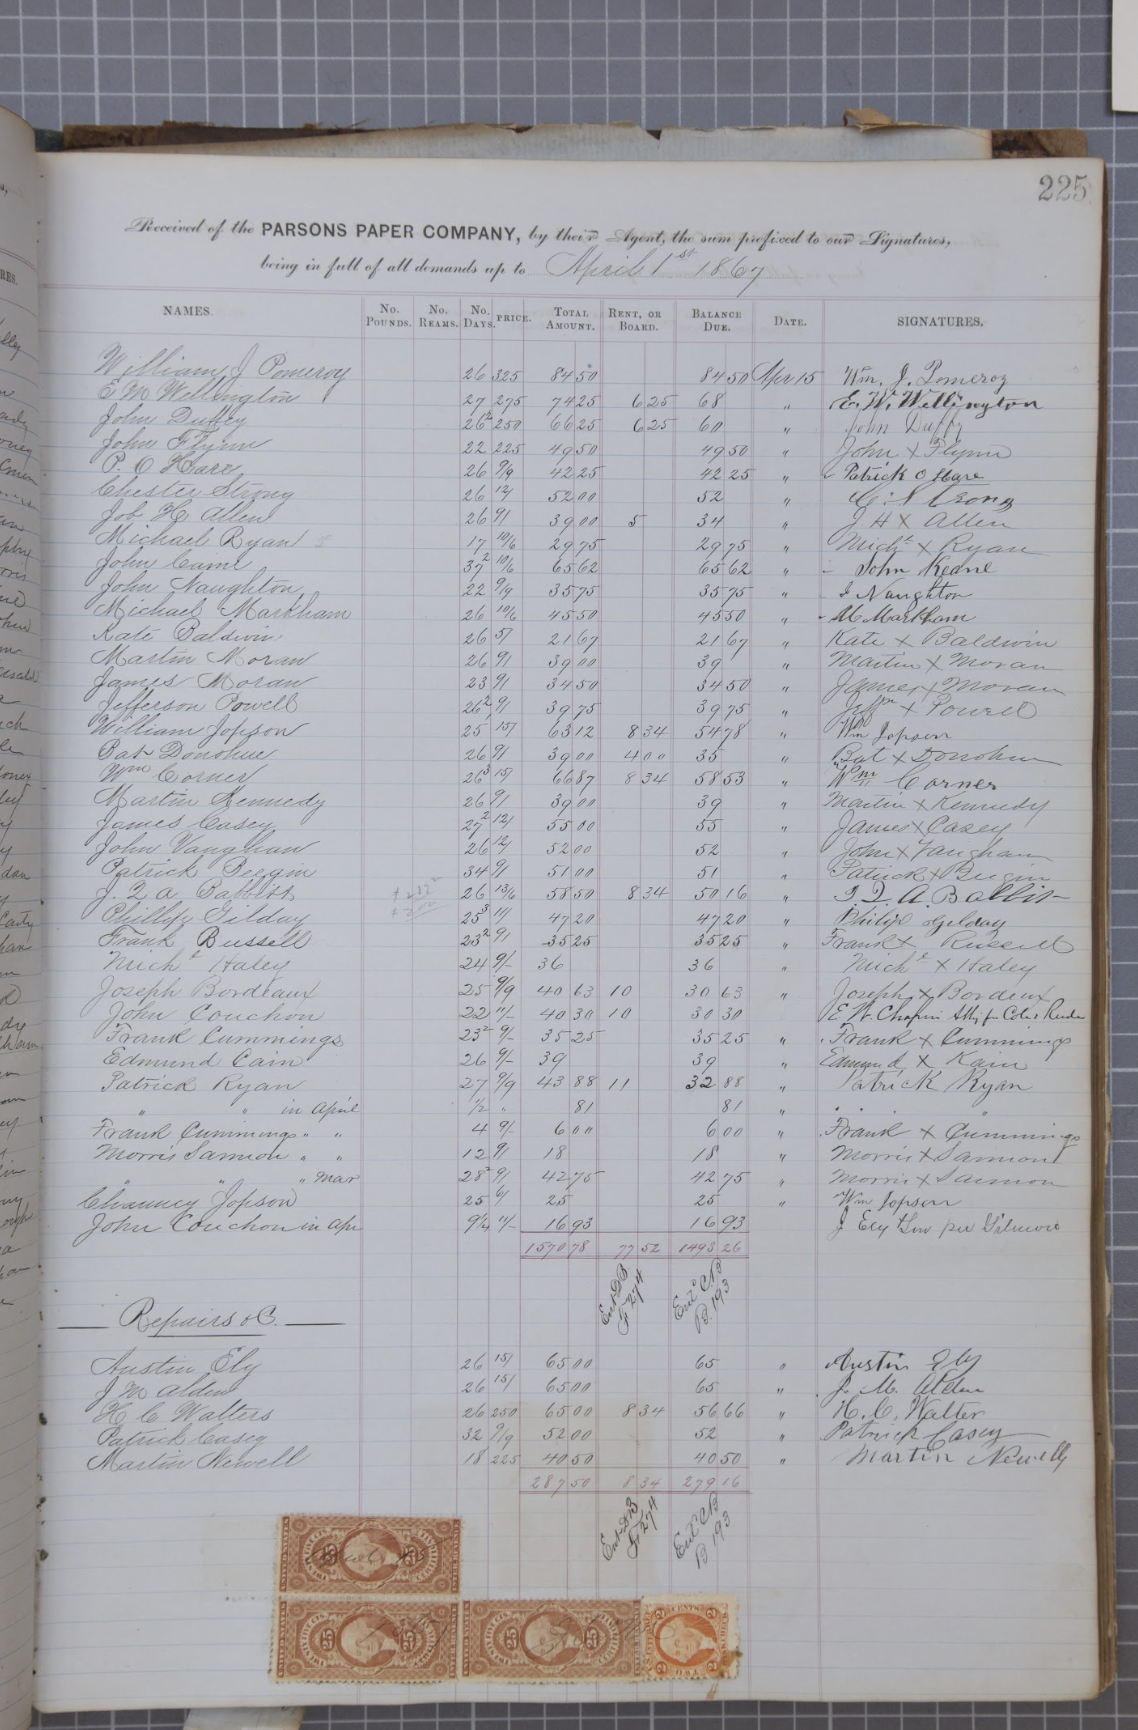
\includegraphics[width=2.29167in,height=\textheight]{images/Screenshot 2023-02-13 at 4.14.16 PM.png}
\end{itemize}

\hypertarget{how-many-employees-during-this-era}{%
\subsection{How many employees during this
era?}\label{how-many-employees-during-this-era}}

\begin{itemize}
\item
  Counted 92 employees in April 1861, 122 employees in April 1862, 141
  employees in April 1863, 128 employees in April 1864, 159 employees in
  April 1865, 144 employees in April 1866, 131 employees in April 1867,
  153 employees in April 1868, 153 employees in April 1869

  \begin{itemize}
  \item
    Average across the measured 9 years = 136 employees between
    1861-1869

    \begin{itemize}
    \tightlist
    \item
      Subset Pages: 8-10 (1861) 43-45 (1862), 79-81 (1863), 115-117
      (1864 - this month also has pay records from the 30th not included
      in the employee count above), 151-153 (1865), 187-189 (1866)
      223-225 (1867), 261-263 (1868), 314-316 (1869)
    \end{itemize}
  \item
    Number of employees generally increased over time

    \begin{itemize}
    \tightlist
    \item
      Green mentions that these mills had abnormally high employee
      retention rates
    \item
      Boom in employment towards end of Civil War in 1865
    \end{itemize}
  \end{itemize}
\item
  Some pages have a separate section of employees at the bottom under
  ``Repairs'' and ``Repairs \& Watchmen'' (April 1862 p.45 - 4 employees
  under `Repairs \& Watchmen') -\/- I included these names in the counts
  above

  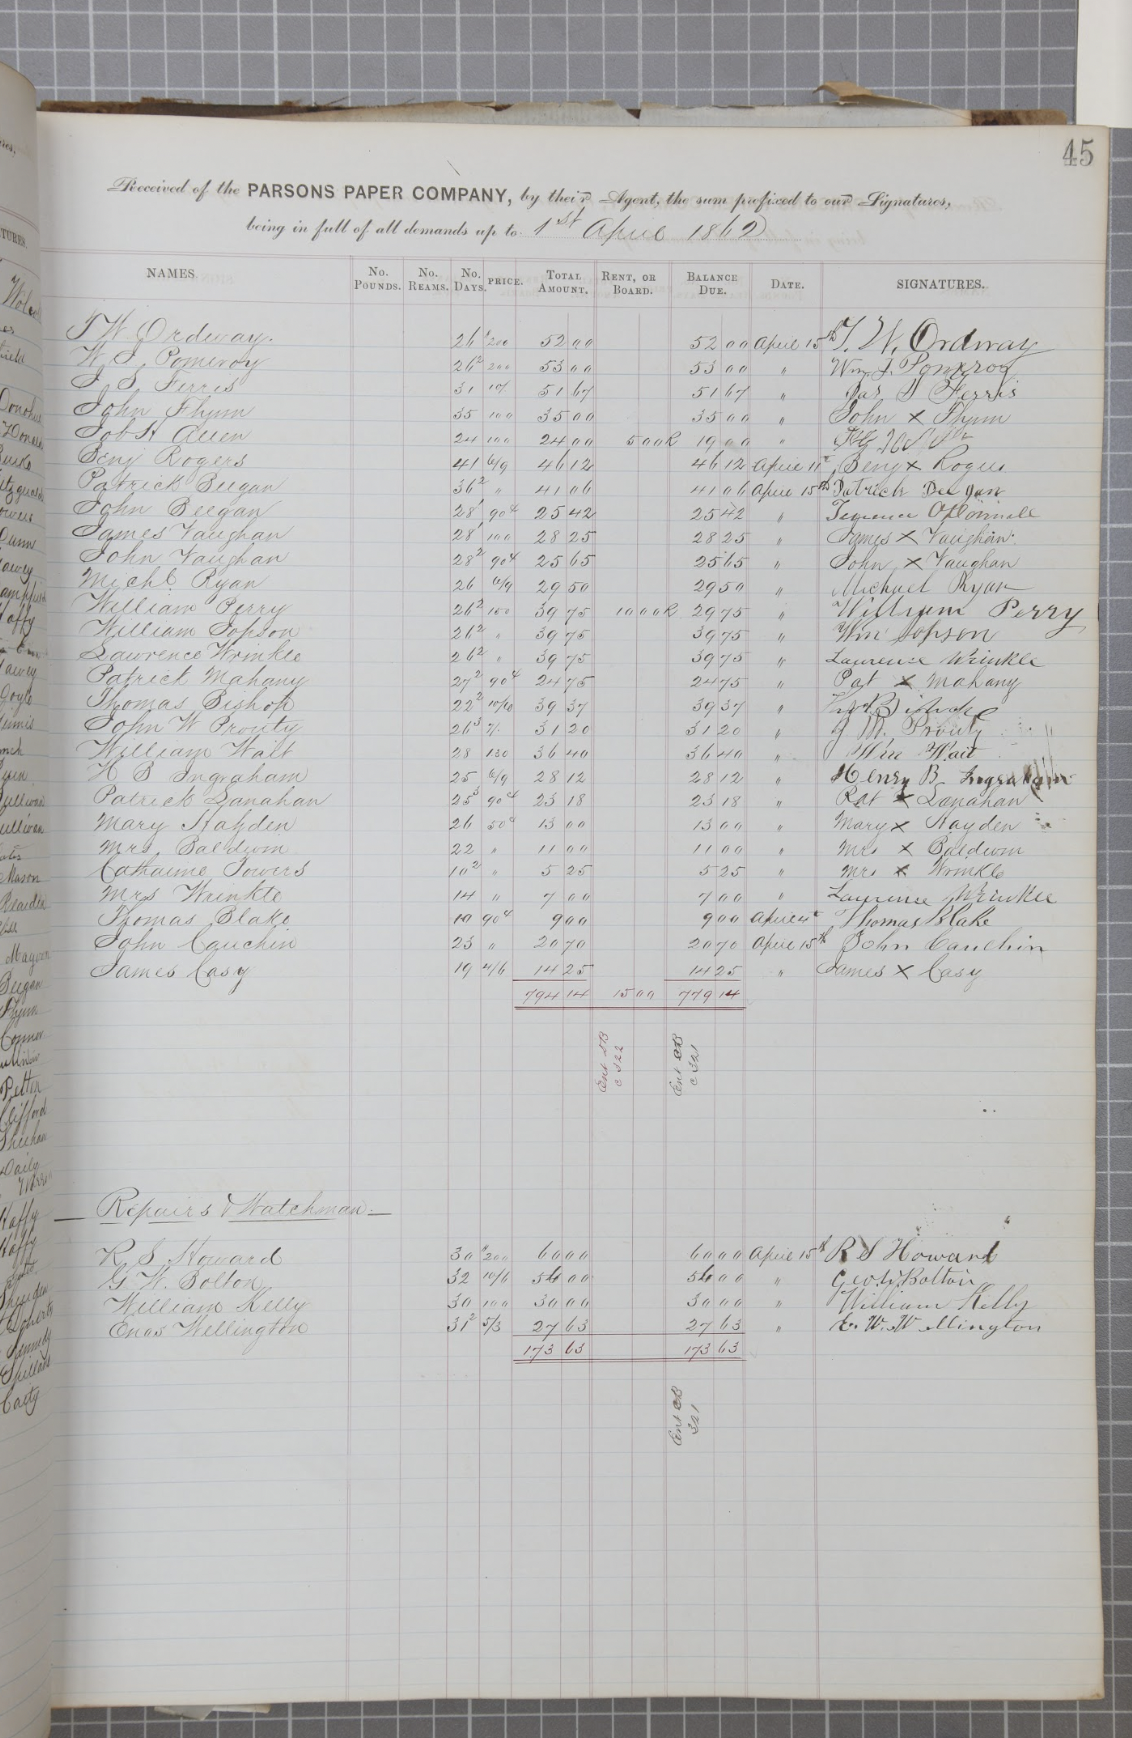
\includegraphics[width=4.20833in,height=\textheight]{images/Screenshot 2023-02-13 at 4.18.46 PM.png}

  \begin{itemize}
  \item
    Presumably employees whose main role was to repair the machines
    instead of making paper
  \item
    There were 5 people under ``Repairs'' for April 1st, 1867 (see
    p.~225 above) and 8 under April 1st, 1868 (see p.~262 above)
  \end{itemize}
\end{itemize}

\hypertarget{what-types-of-jobs-are-there}{%
\subsection{What types of jobs are
there?}\label{what-types-of-jobs-are-there}}

We are listing the roles and the page \# where it is first introduced

\begin{itemize}
\item
  ? (001) - looks like ``MFC'' but we can't decipher it
\item
  repairs (001)
\item
  rag room (002)
\item
  finishers (002)
\item
  ? (005) - looks like something and then ``MFC Mill'' --\textgreater{}
  we googled and found that this is actually the name of a machine
\item
  foreman (005)
\item
  machine room (005)
\item
  engine room (005)
\item
  soft hands (005)
\item
  fireman (005)
\item
  size hands ? (005)
\item
  jobbers ? (005)
\item
  watchmen (005)
\item
  overseer (006)
\item
  day hands (007)
\item
  sorters (007)
\item
  stamp \& sealer (007)
\item
  count \& folder (007)
\item
  engineers (009)
\item
  machine hands (009)
\item
  stamper (011)
\item
  sealer (011)
\item
  sorter (011)
\item
  extra (011)
\item
  borders (013)
\item
  linen ? (021)
\item
  cotton (021)
\item
  cutter (023)
\item
  ? repairs + something else (25)
\item
  repair \& watchmen (030)
\item
  ? SN (034)
\end{itemize}

\hypertarget{spreadsheet-tracking-employment-by-job-type-for-first-6-months-of-the-register-jan-jun-1861}{%
\subsection{Spreadsheet tracking employment by job type for first 6
months of the register (Jan-Jun
1861)}\label{spreadsheet-tracking-employment-by-job-type-for-first-6-months-of-the-register-jan-jun-1861}}

\href{https://docs.google.com/spreadsheets/d/1dza87xBB2pgVajOuLYBM_fHfAobr6IFIZFAu4vFOnhs/edit?usp=sharing}{Spreadsheet
LINK}

\begin{Shaded}
\begin{Highlighting}[]
\NormalTok{employment }\OtherTok{\textless{}{-}} \FunctionTok{read.csv}\NormalTok{(}\StringTok{"jobs.csv"}\NormalTok{)}
\FunctionTok{view}\NormalTok{(employment)}
\end{Highlighting}
\end{Shaded}

\begin{itemize}
\item
  Role labels become very sporadic after first year

  \begin{itemize}
  \item
    `Repairs' and `Repairs and Watchmen', however, remain in their own
    section at the bottom

    \begin{itemize}
    \tightlist
    \item
      All males
    \end{itemize}
  \end{itemize}
\item
  The sorters, stampers, sealers, count\&folders, rag room/cutter roles
  remain throughout 1861-1869, although there are much fewer of them
  compared to the unlabeled names

  \begin{itemize}
  \tightlist
  \item
    These roles were held by almost all women
  \end{itemize}
\end{itemize}

\textbf{Quotes from Hickey thesis that may be of relevance to employment
from 1861-1869}

\begin{itemize}
\item
  ``In 1861, after a period of severe readjustment just prior to the
  Civil War, twenty-one of the thirty-six manufactures of fine papers
  met at Pittsfield\ldots to organize a protrective association. They
  desired to raise prices which had fallen drastically as the result of
  a decrease in demand. They agreed to reduce output by about one-third
  for about three months. This was the first trade association
  established in the paper industry of the United States\ldots.The
  Parsons Paper Company and the Carew Manufacturing Company were charter
  members of this organization'' (108)
\item
  ``Since the discovery of how to utilize wood for the manufacture of
  paper in 1867, this raw material has been in increasing demand'' (84)
\item
  ``several of the local mills were quite large, employing 200 or more
  workers'' and there were ``about 3700 workers employed in the local
  paper industry at the turn of the century'' (4)
\item
  ``Repairs, if necessary, are undertaken on Sundays'' (94)
\item
  ``In replacing a wire on a Fourdrinier paper machine, workers in the
  Holyoke mills receive half a day's pay besides their regular pay
  during the hours they work on the replacement. This acts as an
  incentive to the workers to get the machine back in operation as soon
  as possible'' (94)
\end{itemize}



\end{document}
